\documentclass[11pt]{beamer}
\usepackage[UTF8,scheme=plain]{ctex}
\usepackage{listings}
\usepackage[utf8]{inputenc}
\usepackage[T1]{fontenc}
\usepackage{amsmath}
\usepackage{amsfonts}
\usepackage{amssymb}
\usepackage{graphicx}
\usetheme{Boadilla}

\usepackage{framed} % 可以用 \begin{shaded},即背景色块
\definecolor{shadecolor}{rgb}{0.9,0.9,0.9}

\newcommand{\kong}[1][0.5]{\vspace{#1cm}}

\begin{document}
	\author{ 路毅 \hspace{0.3cm} 曲阜师范大学 }
	\date{\number\year 年 \number\month 月 \number\day 日}
	\title{数学物理方法第五章}

\begin{frame}
	\maketitle
\end{frame}

\kaishu

\begin{frame}{第五章:留数及其应用}
\begin{itemize}
	\item 第一节:留数
	\vspace{1cm}
	\item 第二节:利用留数计算实积分
\end{itemize}
\end{frame}

\begin{frame}{ 圆形围线积分$\oint_C \frac{dz}{(z-a)^n}, n \in Z$ }

\begin{figure}
\centering
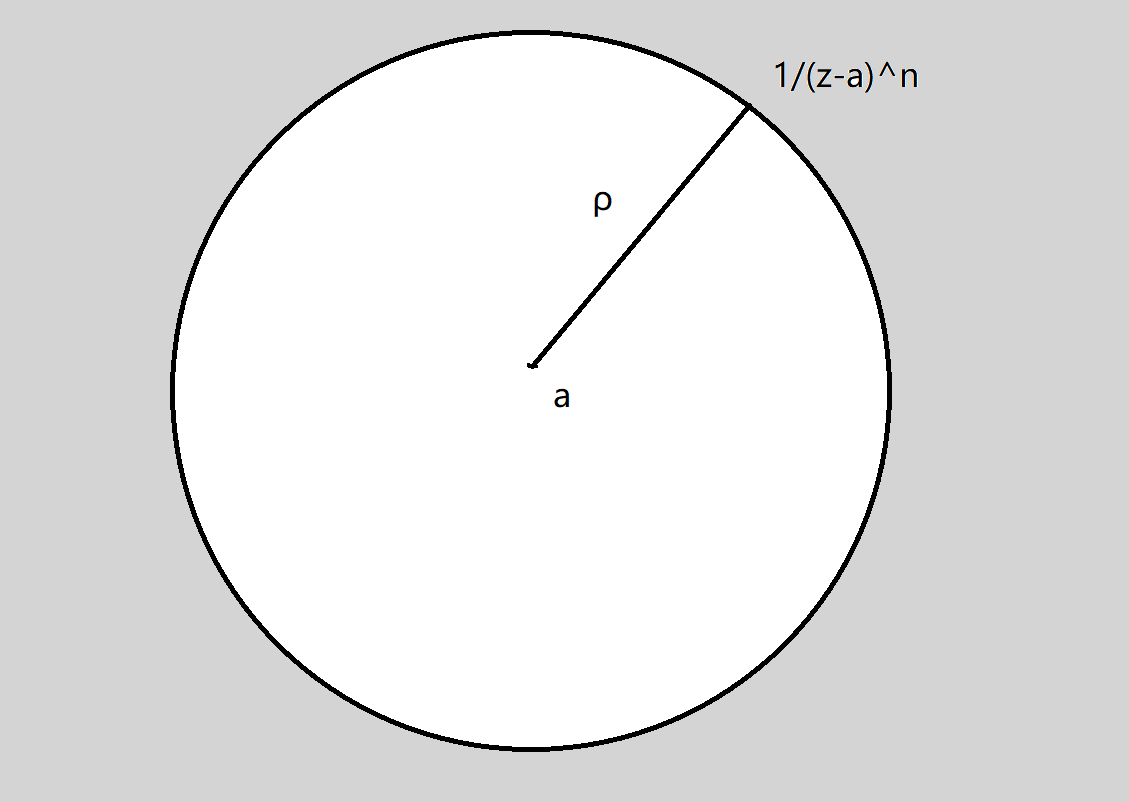
\includegraphics[width=0.4\linewidth]{chap5page1}
\label{fig:chap5page1}
\end{figure}

$C$为半径为$\rho$的圆形围线,$a$为圆心,则可设$z = a + \rho e^{i \phi}$,
\begin{eqnarray}
\oint_C \frac{dz}{(z-a)^n} &=& \int^{2\pi}_0 \frac{i\rho e^{i\phi} d\phi }{(\rho e^{i \phi})^n}
= \int^{2\pi}_0 i \rho^{1-n} e^{i(1-n)\phi} d\phi
\nonumber\\
&=& \left\{
\begin{aligned}
& 2\pi i, ~~ & n=1 \\
& 0, ~~ & else
\end{aligned}
\right.
\end{eqnarray}

\end{frame}

\begin{frame}{任意形状围线积分$\oint_C \frac{dz}{(z-a)^n}, n\in Z$}
\begin{figure}
\centering
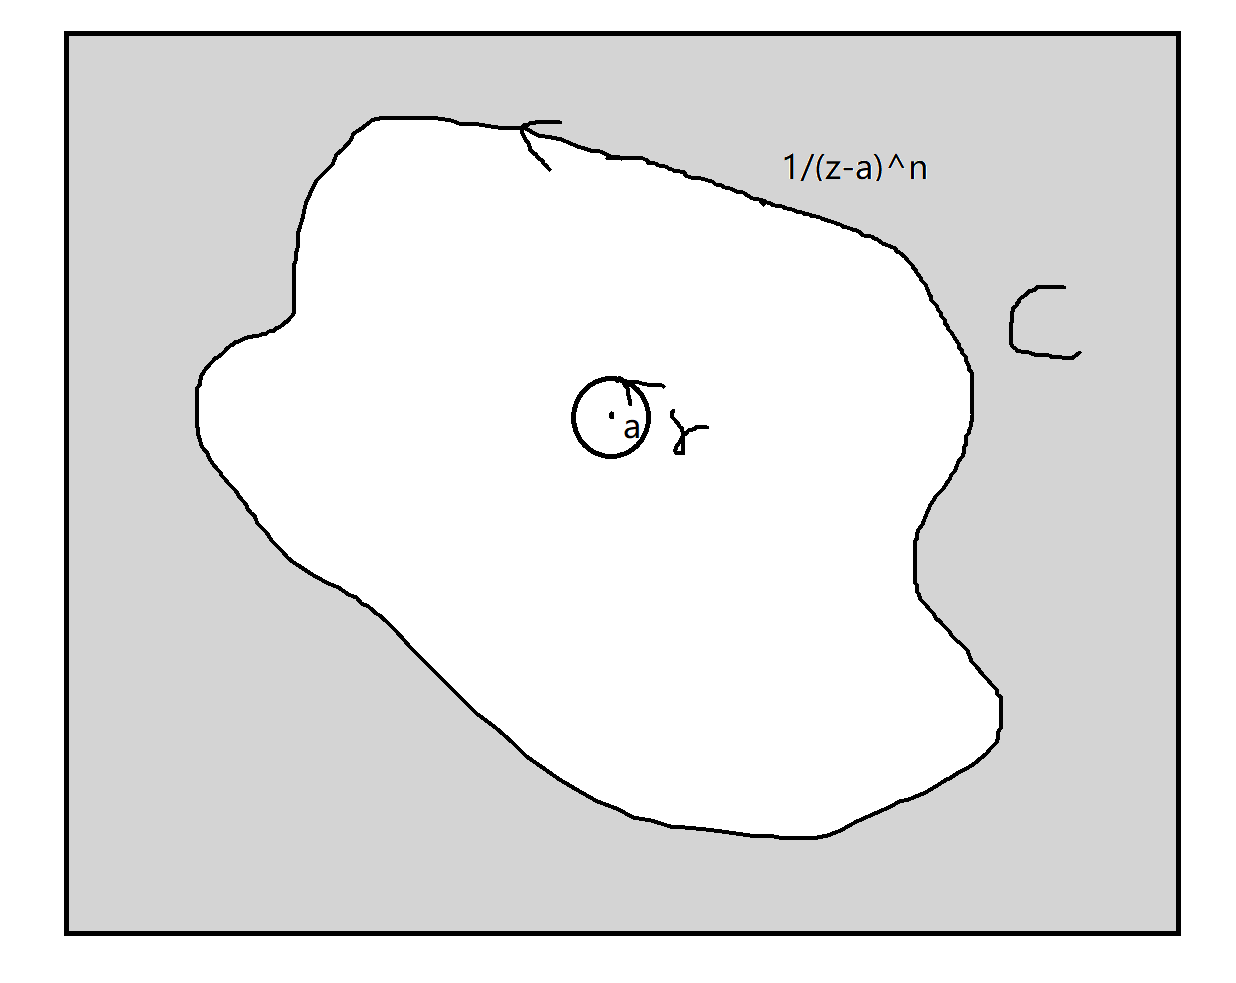
\includegraphics[width=0.4\linewidth]{chap5page2}
\label{fig:chap5page2}
\end{figure}
$C$为任意形状单围线,$a$为其内部一点。
$\gamma$为$C$内部以$a$为圆心的小圆。
根据柯西积分定理,
\begin{equation}
\oint_C \frac{dz}{(z-a)^n} = \oint_\gamma \frac{dz}{(z-a)^n} = \left\{
\begin{aligned}
& 2\pi i, ~~ & n=1 \\
& 0, ~~ & else
\end{aligned}
\right.
\end{equation}

\end{frame}

\begin{frame}{留数:$Res(f,a)=c_{-1}$}
如果解析函数$f(z)$在$a$点的去心邻域$0<|z-a|<R$内洛朗展开为
\begin{equation}
f(z) = \cdots + c_{-2} (z-a)^{-2} + c_{-1}(z-a)^{-1} + c_0 + c_1(z-a) + c_2(z-a)^2 + \cdots,
\end{equation}
$C$为去心邻域内一条围线,$a$点在其内部,则有
\begin{equation}
\oint_C f(z) dz 
= \oint_C \sum_{n=\infty}^{\infty} c_n (z-a)^n dz
= \sum_{n=-\infty}^{\infty} c_n \oint_C (z-a)^n dz
= 2 \pi i c_{-1},
\end{equation}
可见,$\oint_C f(z) dz$完全只关乎$f(z)$洛朗展开的$-1$幂次项系数。

所以,定义 $c_{-1}$ 为函数 $f(z)$ 在 $a$ 点的 {\bf 留数}为:
\begin{equation}
Res(f,a) = c_{-1} = \frac{1}{2\pi i} \oint_C f(z) dz.
\end{equation}
\end{frame}

\begin{frame}{例子}
例1:$f(z)=ze^{1/z}$在本性奇点$z=0$处的留数$Res(f,z=0)$。 

\end{frame}

\begin{frame}{留数定理}
设$f(z)$在围线或复围线$C$所包围的区域$D$内,除点$a_1, a_2, \cdots, a_n$外解析,在闭域$\bar{D}=D+C$上除点$a_1, a_2, \cdots, a_n$外连续,则
\begin{equation}
\oint_C f(z) dz = 2 \pi i \sum_{k=1}^{n} Res(f, a_k),
\end{equation}
证明:
\begin{itemize}
\item [i)] 分别以$a_1, a_2, \cdots, a_n$为圆心作足够小的圆(互相之间无交叠,与$C$无交叠)$\gamma_1, \cdots, \gamma_n$,根据复围线柯西积分定理
\begin{equation}
\oint_C f(z) dz = \sum_{i=1}^n \oint_{\gamma_i} f(z) dz,
\end{equation}
\item [ii)] 根据上页课件,$\oint_{\gamma_i} f(z) dz = 2\pi i Res(f,a_i)$,所以有
\begin{equation}
\oint_C f(z) dz = \sum_{i=1}^n \oint_{\gamma_i} f(z) dz
= 2\pi i \sum^n_{k=1} Res(f, a_k).
\end{equation}
\end{itemize}
\end{frame}

\begin{frame}{留数的求法}
若函数$f(z)$的洛朗展开已知,则取$Res(f,a) = c_{-1}$即可。

\kong[0.5]
定理5.2 若$a$为$f(z)$的$n$阶极点,则
\begin{equation}
Res(f,a) = \frac{1}{(n-1)!} \lim\limits_{z \rightarrow a} \frac{d^{n-1}[(z-a)^n f(z)]}{dz^{n-1}}.
\end{equation}

\kong[0.5]
推论1 若$a$为$f(z)$的一阶极点,则 $Res(f,a) = \lim_{z\rightarrow a} (z-a)f(z)$.

\kong[0.5]
推论2 若$f(z) = \frac{\varphi(z)}{\psi(z)}$, $\varphi(z), \psi(z)$在$a$点解析且$\psi(a)=0, \psi^\prime (a) \neq 0$,则
\begin{equation}
Res(f,a) = \frac{\varphi(a)}{\psi^\prime(a)}.
\end{equation}
\end{frame}

\begin{frame}{例题}
例3 计算$\oint_C \frac{dz}{z^2+1}$,其中$C$为$|z-i|=1, |z+i|=1, |z|=2$。

\kong[0.5]
例4 计算$\oint_{|z|=1} \frac{\cos z}{z^3} dz$。

\kong[0.5]
例5 计算积分$\oint_{|z|=n} \tan (\pi z) dz$,$n$为正整数。

\kong[0.5]
例6 计算$\oint_{|z|=1} \frac{z \sin z}{(1-e^z)^3} dz$。
\end{frame}

\begin{frame}{无穷远点的留数}
定义:设$\infty$为$f(z)$的一个孤立奇点,即$f(z)$在某区域$0\leq r < |z| < \infty$内解析,我们称
\begin{equation}
\frac{1}{2\pi i} \oint_{C^-} f(z) dz ~~ (C:|z|=\rho, \rho \text{充分大})
\end{equation}
为$f(z)$在点 $\infty$的留数,记作$Res(f, \infty)$,$C^-$指沿$C$的顺时针。

若在$|z|$充分大时,$f(z)$有洛朗展开
\begin{equation}
f(z) = \cdots + c_{-n}/z^n + \cdots + c_{-1}/z + c_0 + c_1 z + \cdots + c_n z^n + \cdots,
\end{equation}
可知$ Res(f,\infty) = - c_{-1}$。
\end{frame}

\begin{frame}{所有留数之和为0}
若$f(z)$只有有限个孤立奇点$a_1, \cdots, a_k$,则
\begin{equation}
Res(f,\infty) = \frac{1}{2\pi i} \oint_{C^-} f(z) dz
= - \frac{1}{2\pi i} \oint_{C} f(z) dz
= - \sum_k Res(f,a_k),
\end{equation}
即
\begin{equation}
\sum_k Res(f, a_k) + Res(f, \infty) = 0.
\end{equation}
所有留数之和为零。
\end{frame}

\begin{frame}{例题}
计算积分
\begin{equation}
I = \oint_{|z|=4} \frac{z^{15} dz}{ (z^2+1)^2 (z^4+2)^3 }.
\end{equation}

\kong[1]
思路:
\begin{equation}
I = 2 \pi i \sum_k Res(f,a_k) = - 2 \pi i Res(f, \infty) = 2\pi i c_{-1},
\end{equation}
其中$c_{-1}$为$f(z)$在$|z|$充分大的区域做洛朗展开的$-1$阶系数。 

\end{frame}

\begin{frame}{例题}
例7 计算积分
\begin{equation}
I = \oint_{|z|=4} \frac{z^{15}dz}{(z^2+1)^2 (z^4+2)^3}.
\end{equation}

\kong[1]
思路1:$I= 2 \pi i \sum_k Res(f, a_k) = - 2\pi i Res(f,\infty) = 2 \pi i c_{-1}$,其中$c_{-1}$为$f(z)$在$|z|$充分大时洛朗展开的$-1$阶系数。

\kong[1]
思路2:因为奇点都在$|z|=4$内,所以如果将积分路径改为半径充分大的圆,$I$的值不变,$|z|$充分大时,$f(z) \rightarrow 1/z$,即$I = 2\pi i $。
\end{frame}

\begin{frame}{第二节:利用留数计算实积分}
狄利克雷积分
\begin{equation}
\int^\infty_0 \frac{\sin x}{x} dx.
\end{equation}

\kong[0.5]
菲涅尔积分
\begin{equation}
\int^\infty_0 \sin x^2 dx.
\end{equation}

\kong[0.5]
泊松积分
\begin{equation}
\int^\infty_0 e^{-ax^2} \cos (bx) dx, a>0, b \in R.
\end{equation}
\end{frame}

\begin{frame}{$I = \int^{2\pi}_0 R(\cos\theta, \sin \theta) d\theta$ }
$R( \cos \theta, \sin \theta )$是$\cos \theta, \sin \theta$的二元有理函数,且在$[0,2\pi]$上连续。

\kong[0.5]
在单位圆上有$z=e^{i\theta}, dz = ie^{i\theta}d\theta$,
\begin{equation}
\frac{z + z^{-1}}{2} = \cos \theta,
~~
\frac{z - z^{-1}}{2i} = \sin \theta.
\end{equation}
可以定义
\begin{equation}
f(z) = \frac{1}{iz} R( \frac{z + z^{-1}}{2}, \frac{z - z^{-1}}{2i} ),
\end{equation}
那么$I$可以转化为
\begin{eqnarray}
I &=& \int^{2\pi}_0 R(\cos\theta, \sin \theta) d\theta 
= \int^{2\pi}_0 R(\frac{z+z^{-1}}{2}, \frac{z - z^{-1}}{2i}) d \theta
\nonumber\\
&=& \int^{2\pi}_0 R(\frac{z+z^{-1}}{2}, \frac{z - z^{-1}}{2i}) dz/(iz) 
\nonumber\\
&=& \oint_{|z|=1} f(z) dz = 2\pi i \sum_k Res(f,a_k),
\end{eqnarray}
其中$a_k$为$f(z)$在$|z|=1$内的孤立奇点。
\end{frame}

\begin{frame}{例8}
例8 计算积分
\begin{equation}
\frac{1}{2\pi} \int^{2\pi}_0 \frac{d\theta}{1+\epsilon \cos \theta}, 0< \epsilon < 1.
\end{equation}

\kong[0.5]
思路: 
\begin{equation}
f(z) = \frac{1}{2\pi iz} \frac{1}{1+\frac{\epsilon}{2}(z+z^{-1})}
=\frac{1}{\pi i \epsilon} \frac{1}{z^2 + \frac{2}{\epsilon} z +1}.
\end{equation}
有两个1阶极点
\begin{equation}
z = - \frac{1}{\epsilon} \pm \frac{1}{\epsilon} \sqrt{1-\epsilon^2}.
\end{equation}
一个在单位圆内,一个在单位圆外,取$-1/\epsilon + 1/\epsilon\sqrt{1-\epsilon^2}$处留数,乘以$2\pi i$,即得积分结果。

\end{frame}

\begin{frame}{例9}
计算积分
\begin{equation}
I = \int^{2\pi}_0 \frac{d\theta}{1 - 2p \cos \theta + p^2},
0 <|p|<1.
\end{equation}
思路:
\begin{equation}
f(z) = \frac{i}{pz^2 - (p^2+1)z +p}
=\frac{i}{(pz-1)(z-p)},
\end{equation}
它有两个1阶极点
\begin{equation}
z = p, \frac{1}{p}
\end{equation}
一个在单位圆内,一个在单位圆外,取$z=p$处留数,乘以$2\pi i$即可。
\end{frame}

\begin{frame}{例10}
计算积分
\begin{equation}
I = \int^{2\pi}_0 e^{\cos \theta} \cos(n\theta - \sin \theta) d \theta, n=0,1,2,3,\cdots
\end{equation}
思路:为了方便计算$\cos, \sin$函数,可以给积分补一个虚部部分,构成$e$指数形式,积分完成以后,再取实部,即$I$的值。
\begin{eqnarray}
&& \int^{2\pi}_0 e^{\cos \theta} \cos(n\theta - \sin \theta) d \theta 
- i \int^{2\pi}_0 e^{\cos \theta} \sin(n\theta - \sin \theta) d \theta
\nonumber \\
&=& \int^{2\pi}_0 e^{\cos \theta} e^{-i(n\theta - \sin \theta)} d \theta
= \int^{2\pi}_0 e^{e^{i\theta}} e^{-in\theta} d \theta
\end{eqnarray}
在单位圆上,$z = e^{i\theta}$,所以
\begin{equation}
f(z) = e^z z^{-n} / (iz) = -i e^z z^{-(n+1)},
\end{equation}
有1个$n+1$阶极点$z=0$,留数为$-i/n!$,所以有
\begin{equation}
I = Re \left\{ 2\pi i (-i/n!) \right\} = 2\pi /n!.
\end{equation}
\end{frame}

\begin{frame}{积分路径上无奇点的反常积分$I = \int^\infty_{-\infty}f(x)dx$}
定义:
\begin{equation}
\int^\infty_{-\infty}f(x)dx = \lim_{R \rightarrow \infty} \int^R_{-R} f(x) dx.
\end{equation}
也称作$f(x)$的柯西主值。

构造半圆弧$C: |z|=R, Im z >0$,则有
\begin{equation}
\int^\infty_{-\infty}f(x)dx + \lim\limits_{R \rightarrow \infty} \oint_{|z|=R,Im z>0} f(z) dz = 2 \pi i \sum_k Res(f, a_k),
\end{equation}
其中$a_k$为上半复平面的有限个孤立奇点。

\kong[0.5]
如果$f(z)$确实在上半平面只有有限个孤立奇点,而且上式左边第二项好求,就可以避开直接计算$I$的困难,如上利用留数定理求解。

\end{frame}

\begin{frame}{大圆弧引理}
$f(z)$在圆弧$S_R : z = Re^{i\theta}, \theta_1 \leq \theta \leq \theta_2$($R$充分大)上连续,且
\begin{equation}
\lim\limits_{R \rightarrow \infty} z f(z) = \lambda
\end{equation}
在$S_R$上一致成立,则有
\begin{equation}
\lim\limits_{R \rightarrow \infty} \int_{S_R} f(z) dz = i (\theta_2 - \theta_1) \lambda.
\end{equation}

\end{frame}

\begin{frame}{定理5.5}
设$f(z)$在上半平面$Im z >0$内除了有限多个孤立奇点$a_1, a_2, \cdots, a_n$外解析,在$Im z \geq 0$上除点$a_1, a_2, \cdots, a_n$外连续,且$\lim\limits_{z \rightarrow \infty, Im z \geq 0} zf(z) = 0$一致成立,则
\begin{equation}
\int^\infty_{-\infty} f(x) dx = 2\pi i \sum_{k=1}^{n} Res(f, a_k).
\end{equation}
\end{frame}

\begin{frame}{例题}
例11 设$a>0$,计算$\int^\infty_0 \frac{dx}{x^4 + a^4}$。

\kong[0.5]
例12 计算$I = \int^\infty_{-\infty} \frac{dx}{(x^2+1)^3}$。
\end{frame}

\begin{frame}{若尔当引理}
设$f(z)$在半圆周$\Gamma_R : z=Re^{i\theta}(0 \leq \theta \leq \pi, R \text{充分大})$上连续,且$\lim\limits_{R \rightarrow \infty} f(z) = 0$在$\Gamma_R$上一致成立,则
\begin{equation}
\lim\limits_{R \rightarrow \infty} \int_{\Gamma_R} f(z) e^{imz} dz = 0, (m>0).
\end{equation}
思路:利用若尔当不等式
\begin{equation}
\frac{2\theta}{\pi} \leq \sin \theta \leq \theta, 0 \leq \theta \leq \frac{\pi}{2},
\end{equation}
可以求出
\begin{equation}
\int^{\pi}_0 e^{-mR \sin \theta} d \theta \leq \frac{\pi}{mR}(1-e^{-mR}),
\end{equation}
利用这个式子,可以证明(39)式。
\end{frame}

\begin{frame}{若尔当引理的重要结论}
定理5.6 设$f(z)$在半圆周$\Gamma_R : z=Re^{i\theta}(0 \leq \theta \leq \pi, R \text{充分大})$上连续,且$\lim\limits_{R \rightarrow \infty} f(z) = 0$在$Im z \geq 0$上一致成立,易证
\begin{equation}
\int^\infty_{-\infty} f(x) e^{imx} dx = 2\pi i \sum^n_{k=1} Res(f(z)e^{imz}, a_k), m>0.
\end{equation}
分开等式两边的实部虚部,可得
\begin{eqnarray}
\int^\infty_{-\infty} f(x) \cos(mx) dx &=& - 2\pi Im \left\{ \sum^n_{k=1} Res(f(z)e^{imz}, a_k) \right\},
\\
\int^\infty_{-\infty} f(x) \sin(mx) dx &=& 2\pi Re \left\{ \sum^n_{k=1} Res(f(z)e^{imz}, a_k) \right\}.
\end{eqnarray}
\end{frame}

\begin{frame}{若尔当引理的重要结论}
若$f(x)$为偶函数或奇函数,则
\begin{eqnarray}
\int^\infty_{0} f(x) \cos(mx) dx &=& - \pi Im \left\{ \sum^n_{k=1} Res(f(z)e^{imz}, a_k) \right\},
\\
\int^\infty_{0} f(x) \sin(mx) dx &=& \pi Re \left\{ \sum^n_{k=1} Res(f(z)e^{imz}, a_k) \right\}.
\end{eqnarray}
\end{frame}

\begin{frame}{例题}
例13 计算积分
\begin{equation}
I = \int^\infty_0 \frac{\cos (mx)}{1+x^2} dx, m>0.
\end{equation}
\end{frame}

\begin{frame}{积分路径上有奇点的反常积分}
柯西主值:如果解析函数$f(z)$在$(\alpha,\beta)$上有有限个一阶极点$a_1, a_2, a_3, \cdots, a_n$,则柯西主值定义为
\begin{eqnarray}
&&V.P.\int^\beta_\alpha f(z) dz \\
&&= \lim\limits_{\delta \rightarrow 0} \left\{ \int^{a_1 - \delta}_\alpha f(z) dz
+ \int^{a_2 - \delta}_{a_1 + \delta} f(z) dz
+ \cdots
+ \int^\beta_{a_n + \delta} f(z) dz.
  \right\} \nonumber
\end{eqnarray}

相应地,如果$\alpha = -\infty, \beta = \infty$,则有
\begin{eqnarray}
&&V.P.\int^\infty_{-\infty} f(z) dz \\
&&= \lim\limits_{\delta \rightarrow 0} \left\{ \int^{a_1 - \delta}_{-\infty} f(z) dz
+ \int^{a_2 - \delta}_{a_1 + \delta} f(z) dz
+ \cdots
+ \int^\infty_{a_n + \delta} f(z) dz.
  \right\} \nonumber
\end{eqnarray}
\end{frame}

\begin{frame}{小圆弧引理}

若$f(z)$以$z=a$为一阶极点,则在圆弧$S_r : z-a = re^{i\theta},\theta_1 \leq \theta \leq \theta_2$($r$充分小)上有
$\lim_{r \rightarrow 0 } (z-a) f(z) = c_{-1}$一致成立,其中$c_{-1}$为$f(z)$在$a$点的留数。那么有
\begin{equation}
\lim\limits_{r \rightarrow 0} \int_{S_r} f(z) dz = i(\theta_2 - \theta_1) c_{-1}.
\end{equation}

\end{frame}

\begin{frame}{狄利克雷积分}

\begin{equation}
I = \frac{1}{2} V.P.\int^\infty_{-\infty} \frac{\sin x}{x} dx
= \frac{1}{2}Im \left\{ V.P. \int^\infty_{-\infty} \frac{e^{ix}}{x} dx \right\}.
\end{equation}
考虑图中围线上对$f(z)=\frac{e^{ix}}{2x}$的积分
\begin{figure}
\centering
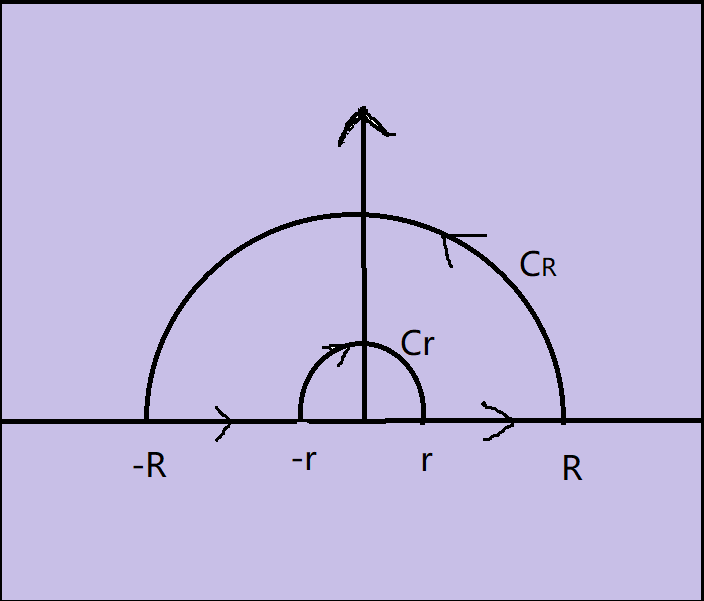
\includegraphics[width=0.5\linewidth]{chap5狄利克雷积分}
\label{fig:chap5狄利克雷}
\end{figure}
\end{frame}

\begin{frame}{狄利克雷积分}
因为$f(z)=e^{iz}/(2z)$在围线及其内部解析,所以由柯西积分定理有
\begin{equation}
\oint_{C_R} f(z) dz - \oint_{C_r} f(z) dz + \int^{-r}_{-R} f(z) dz + \int^R_r f(z) dz = 0,
\end{equation}
取$r \rightarrow 0, R \rightarrow \infty$,得到
\begin{equation}
V.P.\int^{\infty}_{-\infty} f(z) dz = - \lim\limits_{R\rightarrow\infty} \oint_{C_R} f(z) dz + \lim\limits_{r \rightarrow 0} \oint_{C_r} f(z) dz.
\end{equation}
由若尔当引理,
\begin{equation}
\lim\limits_{R\rightarrow\infty} \oint_{C_R} f(z) dz = 0,
\end{equation}
由小圆弧引理,
\begin{equation}
\lim\limits_{r \rightarrow 0} \oint_{C_r} f(z) dz = \frac{\pi}{2}i,
\end{equation}
得到
\begin{equation}
V.P.\int^{\infty}_{-\infty} f(z) dz = \frac{\pi}{2}i,~~
I = Im(V.P.\int^{\infty}_{-\infty} f(z) dz) = \frac{\pi}{2}.
\end{equation}
\end{frame}

\begin{frame}{菲涅尔积分}
\begin{equation}
\int^\infty_0 \sin x^2 dx, \int^\infty_0 \cos x^2 dx,
\end{equation}
定义函数$f(z) = e^{i z^2}$,那么上面的积分即$\int^\infty_0 f(z) dz$的虚部和实部。
取图中的围线,
\begin{figure}
\centering
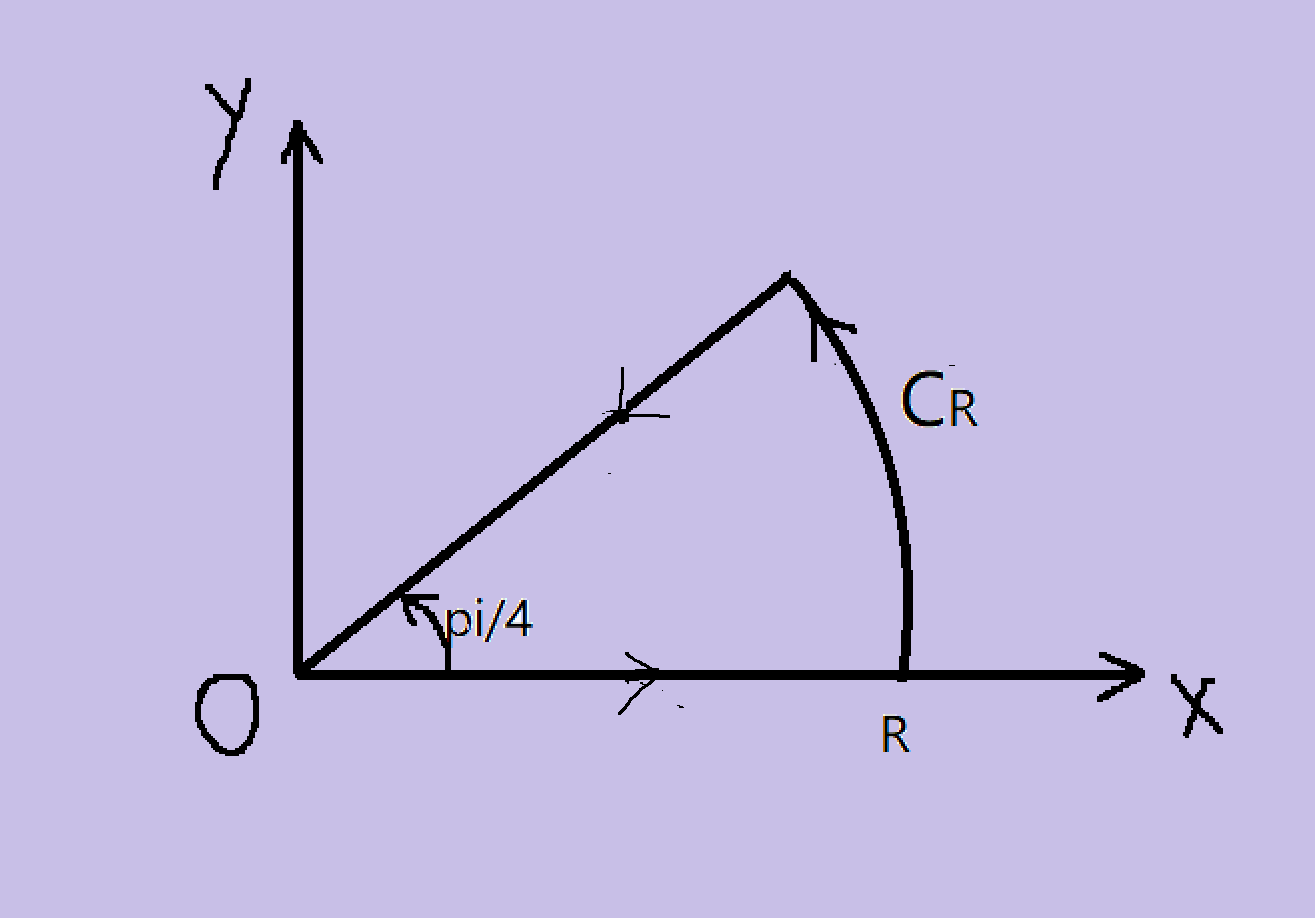
\includegraphics[width=0.5\linewidth]{chap5菲涅耳积分}
\label{fig:chap5菲涅尔}
\end{figure}
\end{frame}

\begin{frame}{菲涅尔积分}
因为 $f(z)=e^{iz^2}$ 处处解析,所以在围线上的积分等于0,即
\begin{equation}
\int^R_0 e^{ix^2} dx + \oint_{C_R} f(z) dz - \int^R_0 e^{i(xe^{i\pi/4})^2} d(xe^{i\pi/4}) = 0,
\end{equation}
即
\begin{equation}
\int^R_0 e^{ix^2} dx + \oint_{C_R} f(z) dz - e^{i\pi/4} \int^R_0 e^{-x^2} dx = 0,
\end{equation}
$R \rightarrow \infty$时,右边第二项为0,可以设$z = Re^{i\theta/2}$,则有
\begin{equation}
|\oint_{C_R} f(z) dz |= |\int^{\pi/2}_0 e^{i(R^2\cos \theta + iR^2 \sin\theta)} (iR/2e^{i\theta/2}) d\theta |
\leq \frac{R}{2} \int^{\pi/2}_0 e^{-R^2 \sin \theta} d\theta
\end{equation}
利用若尔当不等式
$\sin \theta \geq \frac{2}{\pi} \theta,~~ 0<\theta < \pi/2$,
得到
\begin{equation}
|\oint_{C_R} f(z) dz| \leq \frac{R}{2} \int^{\pi/2}_0 e^{-2R^2 \theta/\pi} d\theta = \frac{\pi}{4R}(1-e^{-R^2}) \rightarrow 0.
\end{equation}

\end{frame}

\begin{frame}{菲涅尔积分}
所以,我们从(59)得到
\begin{equation}
\int^\infty_0 e^{ix^2} dx = e^{i\pi/4} \int^\infty_0 e^{-x^2}dx = e^{i\pi/4} \frac{\sqrt{\pi}}{2},
\end{equation}
分别取左右两边的实部、虚部,得到
\begin{eqnarray}
\int^\infty_0 \cos x^2 dx = \frac{\sqrt{\pi}}{2\sqrt{2}}, \\
\int^\infty_0 \sin x^2 dx = \frac{\sqrt{\pi}}{2\sqrt{2}}, \\
\end{eqnarray}

\end{frame}

\begin{frame}{泊松积分}
\begin{equation}
I = \int^\infty_0 e^{-ax^2} \cos(bx) dx, a>0, b\in R.
\end{equation}
可以将$I$补上一个虚部部分
\begin{eqnarray}
I &=& \frac{1}{2}\int^\infty_{-\infty} e^{-ax^2} (\cos(bx) - i \sin(bx)) dx
 = \frac{1}{2}\int^\infty_{-\infty} e^{-ax^2 - ibx} dx
\nonumber\\
&=& \frac{1}{2}e^{-b^2/(4a)} \int^\infty_{-\infty} e^{-a(x+ib/(2a))^2} dx
\end{eqnarray}
这里用到了$\sin(bx)$是奇函数,$\cos(bx)$是偶函数。

\end{frame}

\begin{frame}{泊松积分}
取$f(z) = \frac{1}{2}e^{-b^2/(4a)} e^{-az^2}$, $I = \int^{\infty + ib/(2a)}_{-\infty+ib/(2a)} f(z) dz$。取下图所示围线
\begin{figure}
\centering
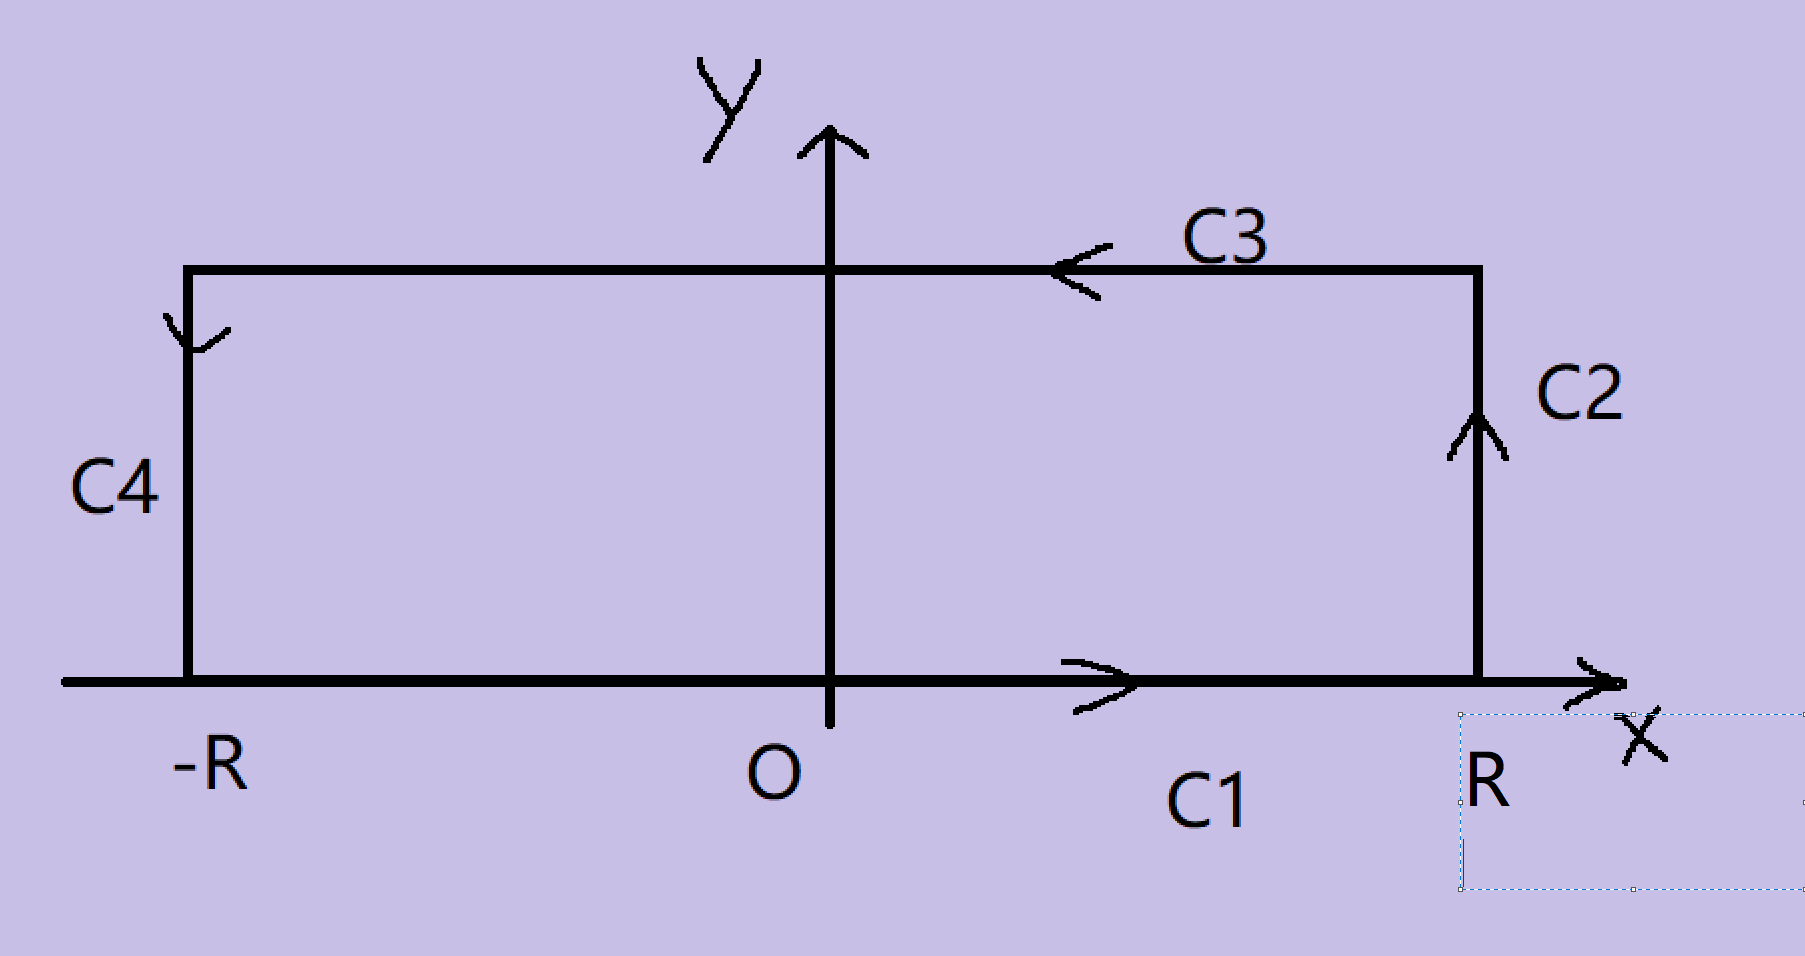
\includegraphics[width=0.5\linewidth]{chap5泊松积分}
\label{fig:chap5泊松积分}
\end{figure}
因为$f(z)$处处解析,所以有
\begin{equation}
\oint_{C_1}f(z) dz + \oint_{C_2}f(z)dz + \oint_{C_3}f(z)dz + \oint_{C_4}f(z) dz = 0,
\end{equation}
$R \rightarrow \infty$时,
\begin{equation}
\oint_{C_1}f(z) dz \rightarrow \frac{\sqrt{\pi}}{2\sqrt{a}}e^{-b^2/(4a)}.
\end{equation}
\end{frame}

\begin{frame}{泊松积分}
\begin{eqnarray}
|\oint_{C_2} f(z) dz| &=& |\frac{1}{2}e^{-b^2/(4a)} \int^{b/(2a)}_0 e^{-a(R+iy)^2} idy|
\nonumber\\
&& \leq \frac{1}{2}e^{-b^2/(4a)} e^{-aR^2} \int^{b/(2a)}_0
e^{a(y)^2} dy \rightarrow 0.
\end{eqnarray}
类似地,$\oint_{C_4}f(z)dz \rightarrow 0$。

另外,$\oint_{C_3}f(z)dz \rightarrow -I$,所以得到
\begin{equation}
I = \oint_{C_1}f(z) dz \rightarrow \frac{\sqrt{\pi}}{2\sqrt{a}}e^{-b^2/(4a)}.
\end{equation}

\end{frame}

\begin{frame}{《庄子》庖丁解牛}
庖丁为文惠君解牛,手之所触,肩之所倚,足之所履,膝之所踦,砉然向(通“响”)然,奏刀騞然,莫不中音。合于桑林之舞,乃中经首之会。

文惠君曰:“嘻,善哉!技盖至此乎?”

庖丁释刀对曰:“臣之所好者道也,进乎技矣。始臣之解牛之时,所见无非牛者。三年之后,未尝见全牛也。方今之时,臣以神遇而不以目视,官知止而神欲行。依乎天理,批大郤,导大窾,因其固然。技经肯綮之未尝,而况大軱乎!良庖岁更刀,割也;族庖月更刀,折也。今臣之刀十九年矣,所解数千牛矣,而刀刃若新发于硎。彼节者有间,而刀刃者无厚;以无厚入有间,恢恢乎其于游刃必有余地矣,是以十九年而刀刃若新发于硎。虽然,每至于族,吾见其难为,怵然为戒,视为止,行为迟。动刀甚微,謋然已解,如土委地。提刀而立,为之四顾,为之踌躇满志,善刀而藏之。”

文惠君曰:“善哉,吾闻庖丁之言,得养生焉。
\end{frame}

\begin{frame}{习题}
\kong[0.5]
课堂选讲:1,3,6

\kong[1]
课下练习:2(1-6),4(1-2),5
\end{frame}

\end{document}